\documentclass{beamer}
\usepackage[utf8]{inputenc}
\usetheme{Madrid}
\usecolortheme{default}
\usepackage{amsmath,amssymb,amsfonts,amsthm}
\usepackage{txfonts}
\usepackage{tkz-euclide}
\usepackage{listings}
\usepackage{adjustbox}
\usepackage{array}
\usepackage{tabularx}
\usepackage{gvv}
\usepackage{lmodern}
\usepackage{circuitikz}
\usepackage{tikz}
\usepackage{graphicx}
\setbeamertemplate{page number in head/foot}[totalframenumber]
\usepackage{tcolorbox}
\tcbuselibrary{minted,breakable,xparse,skins}
\definecolor{bg}{gray}{0.95}
\DeclareTCBListing{mintedbox}{O{}m!O{}}{%
breakable=true,
listing engine=minted,
listing only,
minted language=#2,
minted style=default,
minted options={%
linenos,
gobble=0,
breaklines=true,
breakafter=,,
fontsize=\small,
numbersep=8pt,
#1},
boxsep=0pt,
left skip=0pt,
right skip=0pt,
left=25pt,
right=0pt,
top=3pt,
bottom=3pt,
arc=5pt,
leftrule=0pt,
rightrule=0pt,
bottomrule=2pt,
toprule=2pt,
colback=bg,
colframe=orange!70,
enhanced,
overlay={%
\begin{tcbclipinterior}
\fill[orange!20!white] (frame.south west) rectangle ([xshift=20pt]frame.north west);
\end{tcbclipinterior}},
#3,
}
\lstset{
language=C,
basicstyle=\ttfamily\small,
keywordstyle=\color{blue},
stringstyle=\color{orange},
commentstyle=\color{green!60!black},
numbers=left,
numberstyle=\tiny\color{gray},
breaklines=true,
showstringspaces=false,
}

\title
{9.2.3}
\date{October 6 , 2025}
\author
{EE25BTECH11043 - Nishid Khandagre}

\begin{document}

\frame{\titlepage}

\begin{frame}{Question}
Draw a rough sketch of the given curve $y = 1 + |x + 1|$, $x = -3$, $x = 3$, $y = 0$, and
find the area of the region bounded by them, using integration.
\end{frame}

\begin{frame}{Theoretical Solution}
Given curve
\begin{align}
y = 1 + |x + 1|
\end{align}


For $x < -1$: $|x+1| = -(x+1)$.
    \begin{align}
        y &= 1 - (x+1) \\
        y &= -x
        \end{align}
        \begin{align}
        \myvec{1&1}\myvec{x\\y}=0
    \end{align}

     For $x \ge -1$: $|x+1| = x+1$.
    \begin{align}
        y &= 1 + (x+1) \\
        y &= x+2
        \end{align}
        \begin{align}
        \myvec{1&-1}\myvec{x\\y}=-2
    \end{align}
\end{frame}


\begin{frame}{Theoretical Solution}
At $x=-3$: $y = -(-3) = 3$\\
At $x=-1$: For $y=-x$, $y=1$. For $y=x+2$, $y=(-1)+2=1$.\\Both pieces meet at $\myvec{-1\\1}$\\

At $x=3$: $y = 3+2 = 5$.



The region is bounded by $y = -x$ from $\myvec{-3\\3}$ to $\myvec{-1\\1}$ and $y = x+2$ from $\myvec{-1\\1}$ to $\myvec{3\\5}$ and by the lines $x=-3$, $x=3$, and $y=0$.
\end{frame}

\begin{frame}{Theoretical Solution}
Area calculation for the left piece:\\
For $y=-x$ 
\begin{align}
    \text{Area}_1 &= \int_{-3}^{-1} -x \,dx \\
    &= \myvec{-1 & 0} \left( \myvec{\tfrac{x^2}{2} \\ x} \right) \Big|_{-3}^{-1}
\end{align}

\begin{align}
    \text{Area}_1 &= \left[ -\frac{x^2}{2} \right]_{-3}^{-1} \\
    &= -\frac{1}{2} + \frac{9}{2} \\
    &= 4
\end{align}
\end{frame}

\begin{frame}{Theoretical Solution}
Area calculation for the right piece:\\
For $y=x+2$
\begin{align}
    \text{Area}_2 &= \int_{-1}^{3} (x+2) \,dx \\
    &= \myvec{1 & 2} \left( \myvec{\tfrac{x^2}{2} \\ x} \right) \Big|_{-1}^{3}
\end{align}

\begin{align}
    \text{Area}_2 &= \left[ \frac{x^2}{2} + 2x \right]_{-1}^{3} \\
    &= \left( \frac{9}{2} + 6 \right) - \left( \frac{1}{2} - 2 \right) \\
    &= \frac{21}{2} + \frac{3}{2} \\
    &= 12
\end{align}
\end{frame}

\begin{frame}{Theoretical Solution}
The total area is the sum of the areas of the two pieces.
\begin{align}
    \text{Total Area} &= \text{Area}_1 + \text{Area}_2 \\
    &= 4 + 12 \\
    &= 16
\end{align}
Thus, the total area of the region bounded by the curves is $16$ square units.
\end{frame}

\begin{frame}[fragile]
\frametitle{C Code}
\begin{lstlisting}[language=C]
#include <stdio.h>

// Function to calculate the definite integral of a linear function (mx + c)
double calculate_integral(double m, double c, double a, double b) {
    // Integral of mx + c is (m/2)x^2 + cx
    return ((m / 2.0) * b * b + c * b) - ((m / 2.0) * a * a + c * a);
}
\end{lstlisting}
\end{frame}

\begin{frame}[fragile]
\frametitle{Python Code using C Shared Library}
\begin{lstlisting}[language=Python]
import ctypes
import numpy as np
import matplotlib.pyplot as plt
from matplotlib.patches import Polygon

# Load the shared library
lib_area = ctypes.CDLL("./code15.so")

# Define the argument types and return type for the C function
lib_area.calculate_integral.argtypes = [
    ctypes.c_double,  # m
    ctypes.c_double,  # c
    ctypes.c_double,  # a (lower limit)
    ctypes.c_double   # b (upper limit)
]
lib_area.calculate_integral.restype = ctypes.c_double
\end{lstlisting}
\end{frame}

\begin{frame}[fragile]
\frametitle{Python Code using C Shared Library}
\begin{lstlisting}[language=Python]
# Define the curve function
def f(x):
    return 1 + abs(x + 1)

# Define the integration limits
x_lower_bound = -3
x_upper_bound = 3

# The function y = 1 + |x + 1| needs to be split at x = -1
# For x < -1, x + 1 is negative, so |x + 1| = -(x + 1) = -x - 1
# y = 1 + (-x - 1) = -x
# For x >= -1, x + 1 is positive, so |x + 1| = x + 1
# y = 1 + (x + 1) = x + 2
\end{lstlisting}
\end{frame}

\begin{frame}[fragile]
\frametitle{Python Code using C Shared Library}
\begin{lstlisting}[language=Python]
# Case 1: x_lower_bound to -1 (if -1 is within the bounds)
area_part1 = 0.0
if x_lower_bound < -1:
    lower_limit_1 = x_lower_bound
    upper_limit_1 = min(-1, x_upper_bound) # Ensure we don't go past x_upper_bound
    # For y = -x, m = -1, c = 0
    if lower_limit_1 < upper_limit_1:
        area_part1 = lib_area.calculate_integral(-1.0, 0.0, lower_limit_1, upper_limit_1)

# Case 2: -1 to x_upper_bound (if -1 is within the bounds)
area_part2 = 0.0
if x_upper_bound > -1:
    lower_limit_2 = max(-1, x_lower_bound) # Ensure we don't start before x_lower_bound
    upper_limit_2 = x_upper_bound
    \end{lstlisting}
\end{frame}

\begin{frame}[fragile]
\frametitle{Python Code using C Shared Library}
\begin{lstlisting}
    # For y = x + 2, m = 1, c = 2
    if lower_limit_2 < upper_limit_2:
        area_part2 = lib_area.calculate_integral(1.0, 2.0, lower_limit_2, upper_limit_2)

total_area = area_part1 + area_part2
print(f"The total area bounded by y = 1 + |x + 1|, x = {x_lower_bound}, x = {x_upper_bound}, and y = 0 is: {total_area:.2f}")

# Plotting the curve and the area
x = np.linspace(x_lower_bound - 1, x_upper_bound + 1, 400) # Extend range for better visualization
y = f(x)
fig, ax = plt.subplots(figsize=(10, 6))
# Plot the curve
ax.plot(x, y, 'b', linewidth=2, label=r'$y = 1 + |x + 1|$')
\end{lstlisting}
\end{frame}

\begin{frame}[fragile]
\frametitle{Python Code using C Shared Library}
\begin{lstlisting}
# Plot the boundaries
ax.axvline(x=x_lower_bound, color='gray', linestyle='--', label=f'x = {x_lower_bound}')
ax.axvline(x=x_upper_bound, color='gray', linestyle='--', label=f'x = {x_upper_bound}')
ax.axhline(y=0, color='gray', linestyle='--', label='y = 0')

# Shade the area under the curve
# Create a mask for the region of interest
x_fill = np.linspace(x_lower_bound, x_upper_bound, 200)
y_fill = f(x_fill)
verts = [(x_lower_bound, 0)] + list(zip(x_fill, y_fill)) + [(x_upper_bound, 0)]
poly = Polygon(verts, facecolor='lightgreen', edgecolor='green', alpha=0.5, label='Bounded Area')
ax.add_patch(poly)
\end{lstlisting}
\end{frame}

\begin{frame}[fragile]
\frametitle{Python Code using C Shared Library}
\begin{lstlisting}
# Add annotations for key points
ax.scatter([-1], [f(-1)], color='red', zorder=5, label='Vertex (-1, 1)')
ax.annotate(r'$(-1, 1)$', (-1, f(-1)), textcoords="offset points", xytext=(5,5), ha='left')

ax.set_xlabel('X-axis')
ax.set_ylabel('Y-axis')
ax.set_title(r'Region Bounded by $y = 1 + |x + 1|$, $x = -3$, $x = 3$, and $y = 0$')
ax.grid(True)
ax.legend()
ax.set_ylim(bottom=-0.5) # Ensure y=0 is visible
plt.show()
\end{lstlisting}
\end{frame}

\begin{frame}[fragile]
\frametitle{Python Code: Direct}
\begin{lstlisting}[language=Python]
import numpy as np
import matplotlib.pyplot as plt
from scipy.integrate import quad

# Define the curve
def curve_y(x):
    return 1 + np.abs(x + 1)
# Define the integration function for the area
def integrand(x):
    return curve_y(x)
# Define the limits of integration
x_lower = -3
x_upper = 3
# Calculate the area using numerical integration
area, _ = quad(integrand, x_lower, x_upper)
print(f"The area of the region bounded by the curves is: {area:.2f} square units")
\end{lstlisting}
\end{frame}

\begin{frame}[fragile]
\frametitle{Python Code: Direct}
\begin{lstlisting}[language=Python]
# Generate x values for plotting
x_vals = np.linspace(x_lower, x_upper, 400)
y_vals = curve_y(x_vals)
# Create the plot
plt.figure(figsize=(8, 6))
# Plot the curve y = 1 + |x + 1|
plt.plot(x_vals, y_vals, label=r'$y = 1 + |x + 1|$', color='blue')
# Plot the lines x = -3 and x = 3
plt.axvline(x=x_lower, color='red', linestyle='--', label=r'$x = -3$')
plt.axvline(x=x_upper, color='red', linestyle='--', label=r'$x = 3$')
# Plot the line y = 0 (x-axis)
plt.axhline(y=0, color='red', linestyle='--', label=r'$y = 0$')
\end{lstlisting}
\end{frame}

\begin{frame}[fragile]
\frametitle{Python Code: Direct}
\begin{lstlisting}
# Fill the area under the curve
x_fill = np.linspace(x_lower, x_upper, 400)
y_fill = curve_y(x_fill)
plt.fill_between(x_fill, y_fill, where=(y_fill > 0), color='lightblue', alpha=0.5, label='Bounded Area')

# Add labels and title
plt.xlabel('x')
plt.ylabel('y')
plt.title('Region Bounded by $y = 1 + |x + 1|$, $x = -3$, $x = 3$, $y = 0$')
plt.legend()
plt.grid(True)
plt.axhline(0, color='black', linewidth=0.5)
plt.axvline(0, color='black', linewidth=0.5)
plt.ylim(bottom=0) # Ensure y-axis starts from 0 for clarity of area
plt.show()
\end{lstlisting}
\end{frame}

\begin{frame}{Plot by Python using shared output from C}
\begin{figure}[H]
\centering
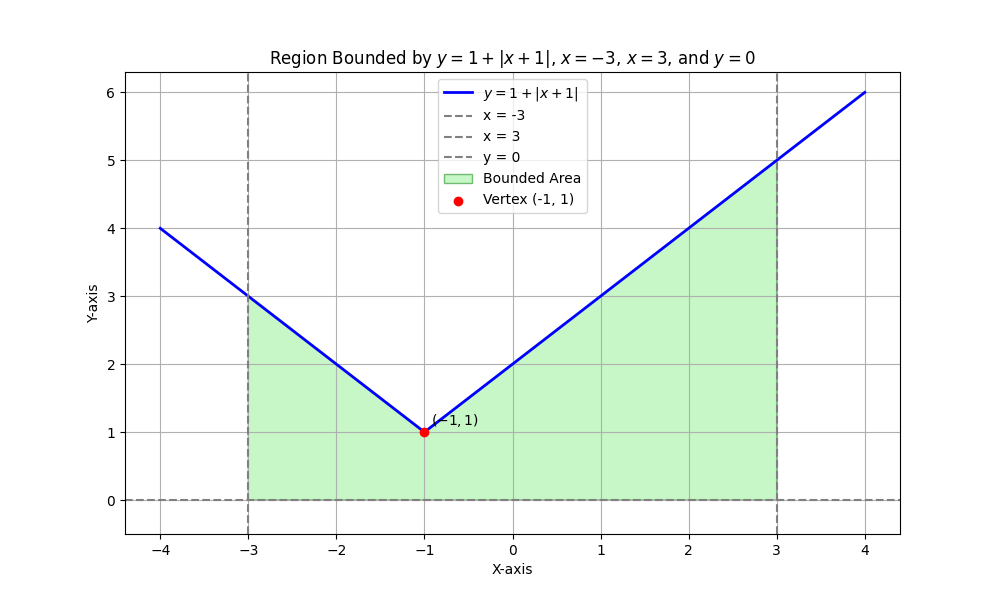
\includegraphics[width=1.0\columnwidth]{../figs/fig1.png}
\caption{}
\label{fig:1}
\end{figure}
\end{frame}

\begin{frame}{Plot by Python only}
\begin{figure}[H]
\centering
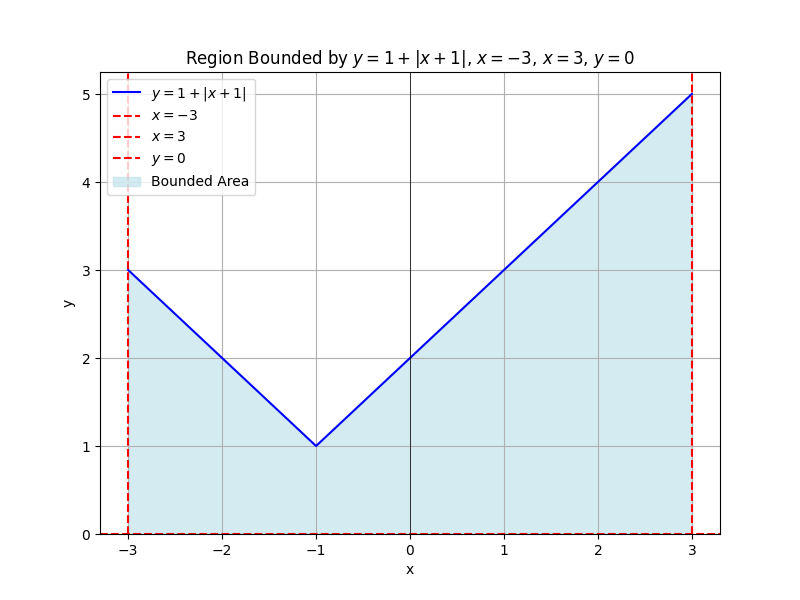
\includegraphics[width=0.7\columnwidth]{../figs/fig2.png}
\caption{}
\label{fig:2}
\end{figure}
\end{frame}

\end{document}
